\documentclass[11pt, oneside]{article}   	% use "amsart" instead of "article" for AMSLaTeX format
\usepackage{geometry}                		% See geometry.pdf to learn the layout options. There are lots.
\geometry{letterpaper}                   		% ... or a4paper or a5paper or ... 
%\geometry{landscape}                		% Activate for rotated page geometry
%\usepackage[parfill]{parskip}    		% Activate to begin paragraphs with an empty line rather than an indent
\usepackage{graphicx}				% Use pdf, png, jpg, or eps§ with pdflatex; use eps in DVI mode
								% TeX will automatically convert eps --> pdf in pdflatex		
\usepackage{amssymb,amsmath}
\usepackage{natbib,verbatim}
\usepackage{hyperref}
\usepackage{aas_macros}

\usepackage{changes}
\definechangesauthor[name=AK, color=blue]{1}

\title{LBL Peculiar-Velocity Program: ZTF2 and LSST}
\author{Alex Kim}
%\date{}							% Activate to display a given date or no date

\begin{document}
\maketitle


%\section{}
%\subsection{}
Measuring peculiar velocities using Type~Ia supernovae is a primary research topic in the upcoming decade.  Peculiar velocities have
been cited as a part of the   Small Projects Portfolio  by the the Cosmic Visions Dark Energy Working Group \cite{2018arXiv180207216D}.

A new group is forming ZTF2, a new 3-year survey using the existing ZTF infrastructure.  We present the case for LBL joining ZTF2.

\section{Probing Gravity With SN~Ia  Peculiar Velocity Surveys}
In the late 1990's, Type~Ia supernovae (SNe~Ia) were used as distance probes to measure the homogeneous expansion history of the Universe.  The remarkable discovery
that the expansion is accelerating  has called into question our basic understanding of the gravitational forces within the Universe.  Either it
is dominated by a ``dark energy'' that is gravitationally repulsive, or General Relativity is inadequate and needs to be replaced by a modified theory of
gravity.  It is only appropriate that in the upcoming decade, with their sheer numbers, solid-angle coverage,
and improved distance precisions, SNe~Ia will provide measurements of the {\it inhomogeneous} motions of structures in the Universe
that will provide an unmatched test of whether dark energy or modified gravity is responsible for the accelerating expansion of the Universe.

In the next decade, SNe~Ia will be used as peculiar-velocity probes to measure  the influence of gravity on structure formation within the Universe.
Peculiar velocities induce scatter along the redshift axis of the SN Hubble diagram, which is
pronounced at low redshifts and when the magnitude scatter (e.g.\ due to intrinsic magnitude dispersion) is small.
The peculiar velocity power spectrum is sensitive to the growth of structure as $P_{vv}\propto (fD)^2$, where $D$ is  the spatially-independent
``growth factor'' in the linear evolution of density perturbations and
$f \equiv \frac{d\ln{D}}{d\ln{a}}$ is the linear growth rate where $a$ is the scale factor  \cite{2006PhRvD..73l3526H,2011ApJ...741...67D}.
The combination $fD$ evolves with redshift;
%\footnote{
%To be precise, the peculiar
%velocity power spectrum also depends on the Hubble parameter as $P_{vv}\propto (HfD)^2$.  A supernova  survey  measures luminosity distance fluctuations
%$\delta_{d_L} = (d_L- \bar{d}_L(z))/\bar{d}_L(z)$, where $d_L$ and  $\bar{d}_L(z)$ are the measured and expected distances at the observed redshift $z$.
%To first order in peculiar velocity along the line of sight $v$, $\delta_{d_L} =  v \left(1-\frac{1}{H\bar{d}_L(z)}\right) \approx -\frac{v}{H\bar{d}_L(z)}$
%at low redshift.   The $H$-dependences of  $P_{vv}$ and the conversion from distances to velocities cancel, making  peculiar velocity surveys sensitive to $(fD)^2$.
%}
the $\Lambda$CDM prediction for the $z=0$ peculiar velocity power spectrum is shown in Figure~\ref{power:fig}.

The  growth of structure depends on gravity;
\cite{2007APh....28..481L} find that General Relativity, $f(R)$,  and DGP gravity follow the relation
$f \approx \Omega_M^\gamma$ with the growth index $\gamma=0.55, 0.42, 0.68$ respectively (see \cite{HUTERER201523} for a review
or these  models).  
Using this parameterization, peculiar velocity
surveys probe  gravity through by modeling $fD=\Omega_M^{\gamma} \exp{\left(\int_a^1 \Omega_M^{\gamma} d\ln{a} \right)}$,
where $\Omega_M(a)$ also depends on the gravity model.
The  $\gamma$-dependence of $fD(z)$ is shown 
in Figure~2 of  \cite{1475-7516-2013-04-031}.

%
%The parameter $\sigma_8$, the  standard deviation of overdensities in 8$h^{-1}$Mpc spheres, is 
%commonly used in place of $D$ to normalize the
%overall amplitude of  overdensities, so the standard parameterization used by the community is $f\sigma_8$.}


\begin{figure}[h]
\centering
\includegraphics[width=0.6\textwidth]{/Users/akim/project/PeculiarVelocity/doc/src/new2.png}
%\includegraphics[width=0.5\textwidth]{../outcosmo/zmax_.png}
\caption{Volume-weighted peculiar velocity power spectrum $k^3P_{vv}(z=0)$ for $\mu \equiv \cos{(\hat{k} \cdot \hat{r})}=1, 0.5$ (magenta, cyan) 
where $\hat{r}$ is the line of sight, as predicted for General Relativity in the linear regime.
Overplotted are peculiar-velocity power-spectrum shot noise  (diagonal lines) for various observing parameters.  Red shows the shot noise expected from a 2-year LSST survey
while black shows a 10-year LSST survey.  The dotted and dashed lines indicate the assumed intrinsic magnitude dispersion, using 0.08 (dashed) or 0.15 mag (dotted).  The expected shot
noise from TAIPAN is shown in green (dash-dotted). 
%
%Overplotted are volume-weighted peculiar velocity shot-noise  $k^3\sigma^2/n$ at $z=0.1$ expected from 2- and 10-year (red, black) supernova densities, 0.08 and 0.15~mag (dashed, dotted) intrinsic magnitude dispersions, and TAIPAN (green, dash-dotted).
The bottom solid grey horizontal lines show the approximate range of $k$ expected to be used in surveys with corresponding
redshift depths $z_{\rm max}$.
\label{power:fig}}
\end{figure}

The same SNe~Ia used  to measure peculiar velocities can also serve as tracers of mass overdensities.  Overdensities and their motions are connected by the
continuity equation, so the SN-overdensity power spectrum also depends on gravity 
as $P_{\delta \delta }\propto (bD + fD\mu^2)^2$ where $b$ is the SN bias and $\mu\equiv \cos{(\hat{k} \cdot \hat{r})}$ where $\hat{r}$ is the direction of
the line of sight.  
The bias is a ``nuisance'' parameter, not present in the velocity power spectrum, which must marginalized out when inferring $\gamma$.
The same field is responsible for both overdensities and velocities so when combined in a common analysis the sample variance limit is lowered.


A SN~Ia peculiar velocity survey is composed of several components:
\begin{itemize}
\item Transient Discoveries -- Wide-field cadenced imaging surveys detect and localize the angular coordinates of new supernovae.
\item Discovery Screening -- Galaxy redshift catalogs, supplemental imaging data can provide subsets of the discoveries for classification
using relatively expensive follow-up resources.
\item SN~Ia Classification -- Spectroscopy classifies the SN~Ia from among the pool of  transient discoveries. 
\item (Host-galaxy) Redshift -- Spectroscopy provides redshifts. 
Host-galaxies generally have more/sharper features that provide more precise redshifts than the supernovae themselves. Resolution $R>200$
is necessary to ensure that statistical uncertainties are negligible.
\item SN~Ia Distance -- Imaging produces photometry and colors for light-curve fitting and getting distances.  The transient search naturally provides some data
for this, of quality that varies depending on the survey strategy.
Spectroscopy and NIR photometry
have been shown to provide more precise distances than with optical light curves alone.
\end{itemize}
The above suite of observations provide a pure sample of SNe~Ia with observed redshifts and cosmological redshifts (inferred from the distances and
the background Hubble law)
whose difference is the radial peculiar velocity.

The precision  in measuring $\gamma$ can be projected for different peculiar velocity surveys.
The primary  parameters that affect the precision are: solid angle $\Omega$, SN number density $n$, source intrinsic
magnitude dispersion $\sigma_M$, and for a distance-limited survey the maximum distance $r_{\text{max}}$ (alternatively redshift $z_{\text{max}}$).
The dependence is most simply discerned 
in the  Fisher information matrix
\begin{align}
F_{ij} 
%& = \frac{V}{2}\int \frac{d^3k}{(2\pi)^3} \text{Tr}\left[ C^{-1} \frac{\partial C}{\partial \lambda_i} C^{-1}
%\frac{\partial C}{\partial \lambda_j} \right]\\
& = \frac{\Omega}{8\pi^2} \int_{r_{\rm min}}^{r_{\rm max}}  \int_{k_{\rm min}}^{k_{\rm max}}  \int_{-1}^{1} r^2 k^2 \text{Tr}\left[ C^{-1} \frac{\partial C}{\partial \lambda_i} C^{-1}
\frac{\partial C}{\partial \lambda_j} \right] d\mu\,dk\,dr
\label{fisher:eqn}
\end{align}
where
\begin{equation}
C(k,\mu)  =
  \begin{bmatrix}
   P_{\delta \delta}(k,\mu) + \frac{1}{n} &
   P_{v\delta}(k,\mu)  \\
   P_{v\delta}(k,\mu)  &
  P_{vv}(k,\mu) + \frac{\sigma^2}{n}
   \end{bmatrix},
\label{cov:eq}
\end{equation}
and $\sigma \approx (\frac{5}{\ln{10}} \frac{1+z}{z})^{-1} \sigma_M$.
The dependences of $\gamma$ and other parameters enter through $fD$ in the relations $P_{vv}\propto (fD\mu)^2$, the SN~Ia host-galaxy count overdensity
power spectrum $P_{\delta \delta }\propto (bD + fD\mu^2)^2$, and the galaxy-velocity cross-correlation $P_{vg}
\propto  (bD + fD\mu^2)fD$.  
 The density and velocity covariances depend on the parameter set $\lambda \in \{\gamma, \Omega_{M0}, b\}$.
Taking $\Lambda$CDM as our fiducial model, 
$\Omega_M=\frac{\Omega_{M_0}}{\Omega_{M_0} + (1-\Omega_{M_0})a^3}$.  
The uncertainty in the growth index is bounded by $\sqrt{F^{-1}_{\gamma \gamma}}$.

\section{Current Results and Projections}
\subsection{Current Results}
Peculiar velocity surveys have already been  used to measure
the effective $fD$ in redshift bins  (referred to as $f\sigma_8$), though not to a level where  gravity models can be precisely distinguished.
 \cite{2017MNRAS.471..839A} use 6dFGS peculiar velocities using  Fundamental Plane distances of elliptical galaxies to estimate absolute magnitudes
 with
 $\sim 0.43$~mag  precision, yielding a 15\% uncertainty in $fD$ at $z\approx 0$.
The upcoming 
TAIPAN survey \cite{2017PASA...34...47D} will obtain Fundamental Plane galaxies with densities of $n_g \sim 10^{-3}h^3$\,Mpc$^{-3}$,
and the WALLABY+WNSHS surveys \cite{2008ExA....22..151J} will obtain Tully-Fisher distances (based on the $\sim 0.48$~mag calibration of absolute magnitude based on the  HI 21cm line width)
of galaxies with densities $n_g \sim 2\times 10^{-2} - 10^{-4} h^3$\,Mpc$^{-3}$ from
$z=0-0.1$ covering 75\% of the sky.
These surveys combined are projected to have 3\% uncertainties in $fD$ \cite{2017MNRAS.464.2517H}.
For reference, DESI projects a 10\% precision of $fD$ at $z \approx 0.3$  by looking 
for signatures (Redshift Space Distortions; RSD) expected from galaxies infalling toward mass overdensities.
Relative to galaxies with  Fundamental Plane or Tully-Fisher distances, 
SN~Ia host galaxies currently have significantly lower number density but have better per-object peculiar velocity precision.
Existing SN~Ia samples
have been used to test and ultimately find spatial correlations in peculiar velocities that may be attributed to the growth of structure
\cite{PhysRevLett.99.081301,2008MNRAS.389L..47A,2014MNRAS.444.3926J,2015JCAP...12..033H, 2017JCAP...05..015H}.
SNe~Ia discovered by ASAS-SN, ATLAS, and ZTF \cite{2014ApJ...788...48S,2018PASP..130f4505T,2019PASP..131a8002B} over the next several years will provide first probative measures of $fD$ at $z<0.1$.
%Measurement of the velocity field using LSST-discovered
%SNe~Ia has been quantified by \cite{2011PhRvD..83d3004B,2017JCAP...01..060O}

\subsection{Projections}
Two advances in the upcoming decade will make SN~Ia peculiar velocities more powerful.
First, the precision of SN~Ia distances can be improved.  The commonly-used empirical 2-parameter spectral model yields  absolute magnitude
dispersion $\sigma_M \gtrsim 0.12$~mag.  However, SNe transmit more information than just the light-curve shape and single color used in current SN models.
Recent studies indicate that with the right data, SN absolute
magnitudes can be calibrated to $\sigma_M \lesssim 0.08$ mag \cite[see e.g.][]{2012MNRAS.425.1007B, 2015ApJ...815...58F}. 
Though not yet
established, it is anticipated that such a reduction in intrinsic dispersion comes with a reduction in the magnitude bias correlated with host-galaxy properties
that is observed using current calibrations.  At this precision the intrinsic velocity dispersion  at $z=0.028$ is  $300$~km\,s$^{-1}$, i.e.\ a single SN~Ia  is of such quality as to
measure a peculiar velocity with $S/N \sim 1$.
 If corrections of all SNe~Ia are not possible, the use of SN~Ia subclasses is an option though at the expense of reducing the
numbers of velocity probes.
Secondly,  in the upcoming decade cadenced wide-field imaging surveys such as ZTF2 and LSST
  will increase the number of identified  $z<0.2$ Type~Ia supernovae from the hundreds to the
hundreds of thousands; over the course of 10-years, LSST will find $\sim150,000$ $z<0.2$ SNe~Ia
 for which good light curves can be measured, corresponding to a  number density of $n \sim 5\times 10^{-4}h^3$\,Mpc$^{-3}$.
  This sample has comparable
 number density and more galaxies at deeper redshifts than projected by WALLABY and TAIPAN.  With similar densities,
 the (two) ten-year SN~Ia survey will have
 a (6) 29$\times$ reduction in shot-noise, $\sigma^2_M/n$, relative to the Fundamental Plane survey of TAIPAN.

A SN~Ia peculiar velocity program hinges on  SN discoveries, the number density $n$ of which
depends on the cadenced wide-field imaging survey used for the search.    
It is thus convenient to make projections for upcoming programs
based on the imaging survey; the projections here use ZTF2 and LSST 
as canonical representatives.
Keep in mind that other follow-up resources determine the distance precision $\sigma_M$, the another important parameter
that affects projections.


The primary sources of systematic error in a high-redshift supernova Hubble diagram are not as important for a low-redshift
peculiar velocity survey.  A Hubble diagram that spans a broad redshift range requires absolute color calibration over the corresponding observer-frame
wavelength range and control over the different populations over the span of cosmic time from which SNe are drawn.  High-redshift peculiar
velocity measurements do not have much sensitivity to $\gamma$, and a SN survey confined to lower redshifts are less sensitive to
color-calibration uncertainties and population evolution.

Details on the assumptions made for the calculations that follow can be found in \cite{2019BAAS...51c.140K}.

\subsubsection{Near-Term: ZTF2}
ZTF2 and TAIPAN are near-term surveys that will measure peculiar velocities, the former using SNe~Ia and the latter
using Fundamental Plane Galaxies.  Both have roughly
 $z_{\text{max}}=0.09$ and $\Omega = 2\pi$.
Uncertainties in $\gamma$ for surveys with this depth and solid-angle coverage 
are shown as a function of number of sources $N$ and $\sigma_M$ in Figure~\ref{surface:fig}. 

The positions of ZTF2 and TAIPAN are marked
in the figure, with the latter showing both  a conservative $\sigma_M=0.12$~mag and aggressive $\sigma_M=0.08$~mag.
The former is the uncertainty that could be achieved with ZTF2 photometry alone, the latter with additional
SN follow-up.
ZTF2 and TAIPAN lie in opposite ends of the figure, there are small numbers of ZTF2 SNe with precise distances
whereas there are many TAIPAN Fundamental Plane galaxies with imprecise distances. 
Conservative ZTF2 and TAIPAN
are projected to give similar precisions $\sigma_ \gamma = 0.053$, whereas  aggressive ZTF2 gives a more constraining
$\sigma_ \gamma = 0.043$.  
Recall that the difference in $\gamma$  between GR and the $f(R)$ and DGP gravity is 0.13, meaning that the surveys
can already distinguish between these models to $2-3 \sigma$.

\begin{figure}
\centering
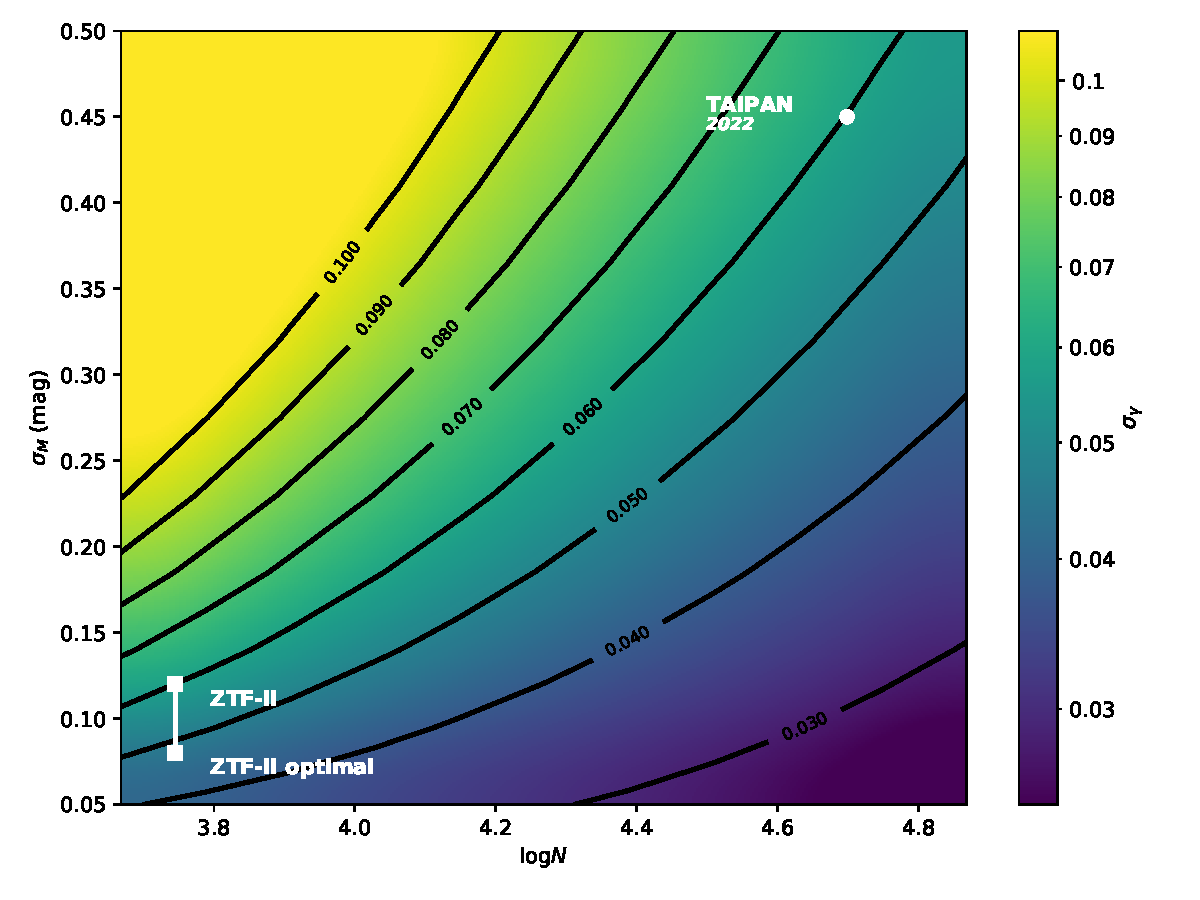
\includegraphics[width=0.6\textwidth]{src/surface1.pdf}
\caption{Uncertainties in $\gamma$ for surveys  with $z_{\text{max}}=0.09$ and $\Omega = 2\pi$
are shown as a function of number of sources $N$ and $\sigma_M$.  The positions of ZTF2 and TAIPAN are marked,
with the latter showing both  a conservative $\sigma_M=0.12$~mag and an aggressive $\sigma_M=0.08$~mag.
\label{surface:fig}}
\end{figure}

An important distinction between the surveys is
that TAIPAN will observe almost all available Fundamental Plane galaxies in the local volume, meaning that no additional observing can
increase the number density $n$ and decrease $\sigma_\gamma$.  On the other hand, the number density of supernova increases
linearly with time, there is continued room for decreased $\sigma_\gamma$ with longer surveys  as ZTF2 is not  sample-variance limited 


ZTF2 and TAIPAN are not in competition but are complementary.  Being in different hemispheres, the two surveys
cover different parts of sky, meaning that their two independent results can be
combined  quadratically to produce a reduced joint uncertainty. 

\subsubsection{Long-Term: LSST}
A long-term supernova peculiar-velocity survey can be performed with SNe~Ia discovered by LSST.
As a 10-year survey, LSST generates higher supernova number densities to fainter limiting magnitude than  ZTF2,
making possible significantly improved constraints on the growth index.
All the proposed LSST surveys have complete SN~Ia discovery out to $z=0.3$.
The expected distance uncertainties derived from LSST light curves vary greatly depending on observing strategy, but at best
is expected to be $\sigma_M=0.12$~mag.    As with the ZTF2 survey,  lower magnitude uncertainties
can be achieved with supplemental data.

Uncertainties in $\gamma$ for surveys with a 10-year duration   and $\Omega=2\pi$ sky coverage, applicable to the LSST WFD survey, 
are shown as a function of imiting  redshift $z_{max}$ and $\sigma_M$ in Figure~\ref{lsst:fig}.
The redshift depth afforded by LSST provides significant improvement relative to the shallower ZTF2 survey.
After 10 years, the region with $z_{max}<0.1$ has $\sigma_\gamma$ that is only weakly $\sigma_M$-dependent, 
which reflects the relatively strong sample variance in the small local survey volume.  
As $\sigma_\gamma$ quickly increases for surveys shallower than the $z_{\text{max}}=0.09$ 
of ZTF2,
better growth index constraints
are achieved by going to $z_{max}>0.1$.
The gradient in decreasing $\sigma_\gamma$ does shallow out with increasing redshift despite the increased survey volume, 
as the velocity uncertainties degrade with redshift for a fixed $\sigma_M$.

\begin{figure}
\centering
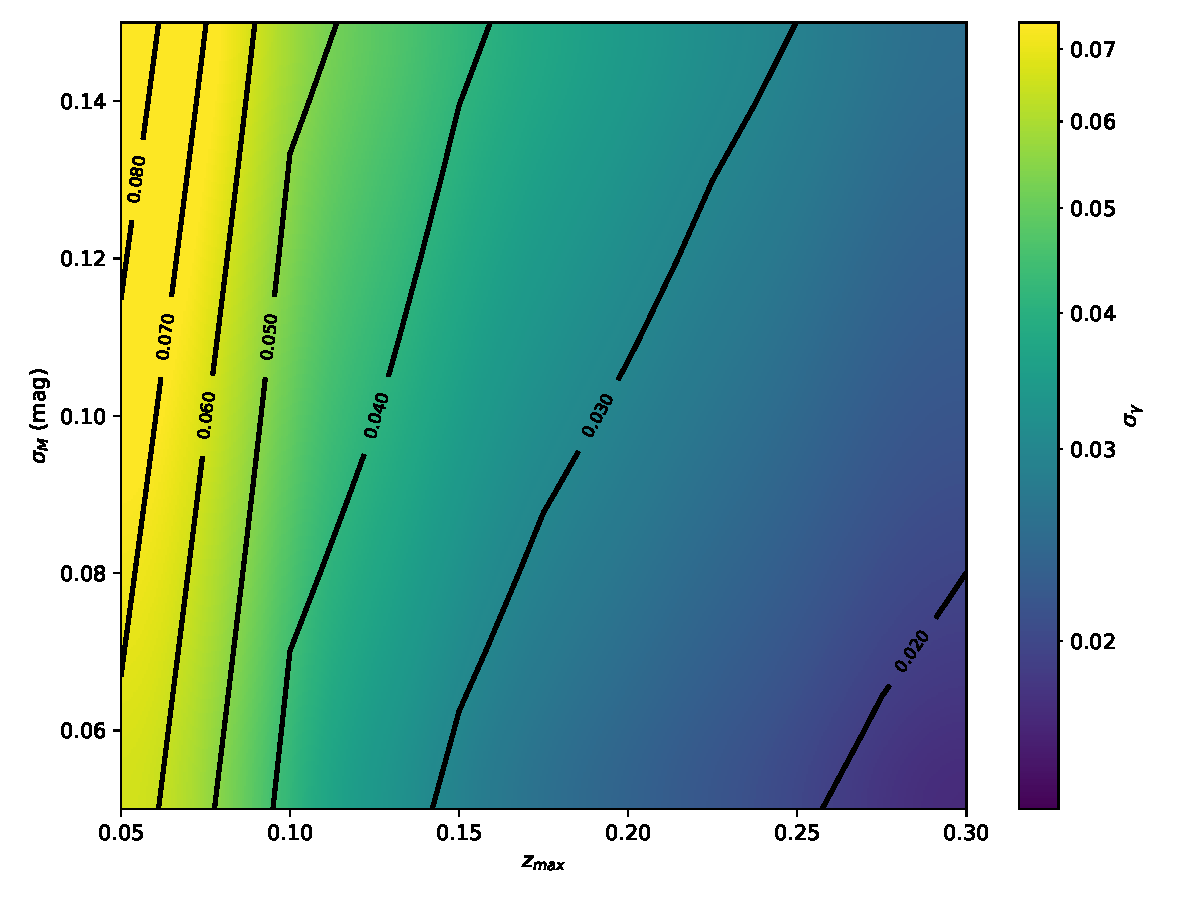
\includegraphics[width=0.6\textwidth]{src/surface2.pdf}
\caption{Uncertainties in $\gamma$ for surveys with a 10-year duration and  and $\Omega=2\pi$ sky coverage 
are shown as a function of limiting  redshift $z_{max}$ and $\sigma_M$.
\label{lsst:fig}}
\end{figure}

\subsection{Complementarity with High-$z$ redshift surveys}
Combined low-redshift peculiar velocity and high-redshift RSD $fD$ measurements (i.e.\ from DESI) are highly complementary as together they probe the
$\gamma$-dependent shape of $fD(z)$ (not just its normalization) and potential scale-dependent influence of gravitational models, since low-
and high-redshift surveys are weighted by lower and higher $k$-modes respectively.

\section{Plan for a Peculiar Velocity Program}
The projections for measuring $\gamma$ with ZTF2 and LSST SN~Ia discoveries
show the power of peculiar velocities surveys at low redshift.
This  tracer provides an unmatched  new window with which to test gravity and the source of the accelerating expansion of the Universe.
We propose the following course of research for the upcoming decade.

\subsection{Present}
The current goals are to provide a proof of concept of a SN peculiar velocity survey while developing domain
expertise and pipelines that can be used in future experiments.

Kim has developed a SNFactory/ZTF postdoc on a peculiar-velocity analysis framework.  Its distinguishing features is that it is likelihood-based
including both density and peculiar velocities.  The complexity of including the underlying mass density field as a latent layer in the model
is addressed through Hamiltonian Monte Carlo.  Analytic expressions for the partial derivatives of the likelihood are coded,
avoiding the computational limitations of {\it autodiff} in STAN.  A end-to-end implementation is complete, validation of it is ongoing.

The first application o the analysis pipeline will be for SNFactory supernovae.  A next analysis will be of ZTF-discovered 
SNe when those data are ready.  The plan is for a  subset of the required data, precision redshifts of SN host galaxies, to be provided
by DESI.  Additional DESI data contributions are being discussed.

\subsection{Near Term: DESI as TAIPAN-North}

There has been talk of using BGS for a peculiar-velocity survey.  There is some question as to how deep the BGS achieves.  This should be
dug into.

\subsection{Near Term: ZTF2 + DESI}
A near-term peculiar velocity program can already provide the most competitive measurements of $\gamma$ at low redshift.  Engaging in science
now positions LBL for domain leadership in the LSST era.  For its near-term peculiar-velocity program, we advocate a survey using SN~Ia discoveries from ZTF2,
rather than other possible surveys, for the following reasons:
\begin{itemize}
\item A peculiar-velocity survey is already being touted as a primary science driver. As such,
the observing strategy should accommodate our needs.
\item It would be ready to start at the end of ZTF in 2021.
\item It is cheap, with a cost ranging from zero to access public data, to an amount (\$300k?) smaller
than building a new facility.
\item ZTF2 includes SEDMachine for classification of $m<18.5$ transients.
\item It is in the Northern Hemisphere, which complements and is not superseded by LSST. 
Even after the nominal 3-year survey and simultaneous with LSST, the facility remains important for peculiar-velocity studies.
\item It is anticipated that the public plus private collaboration surveys can be designed to generate distance
precisions of $\sigma_M =0.12$~mag, which allow good velocity measurements with SNe~Ia.  (Additional follow-up can lower this uncertainty further.)
\item The limiting redshift $z_{\text{max}} =0.09$ is sufficiently deep  to have a scientifically interesting result $\sigma_\gamma < 0.053$.
There are other SN searches that do not achieve this depth.
\end{itemize}

ZTF2 SN~Ia discoveries are combined with data from other facilities to form a complete PV program.  We propose:
\begin{itemize}
\item DESI will provide the following components of the survey:
\begin{itemize}
\item Discovery Screening -- Provides redshifts for probable host galaxies of new transients, for use in early classification.  A host galaxy may
already have a DESI redshift, may be a BGS target without a redshift but whose observation could be prioritized,  or non-DESI target for which we
make a secondary-target fiber allocation.
\item SN Ia Classification -- Spectroscopy of active transients  through secondary-target fiber allocations within
DESI survey pointings. There
will be $\sim 1$ active $r<21.5$ SN~Ia in every three DESI pointings.  Coordinating DESI pointings such that ``every'' pointing contains
a  ZTF2 discovery can significantly increase the number of classifications, relative to the random (from the transient perspective) default DESI pointings.
Triggered observations of non-DESI pointings is possible, though does not take advantage of DESI multiplexing.
\item Host-galaxy redshift -- Some precise galaxy redshifts may not be available at the end of the ZTF2 survey.  Mopping up of ZTF2 host-galaxy redshifts
can be done efficiently with a single sweep of DESI's MOS.
\end{itemize}
 The $R>2000$ resolution
provides sufficiently precise redshifts so as to make their uncertainties negligible in the $\gamma$ error budget.
Its BGS targets  will host a large fraction of ZTF2-discovered SNe~Ia.
\item SNIFS at the UH-88 is used to spectroscopically observe a subset of active likely-SN~Ia transients.  SNIFS provides simultaneously
\begin{itemize}
\item SN Ia Classification -- SNIFS can supplement SED Machine to go toward 100\% SN~Ia classifications
while going deeper than the nominal $18.5$~mag limit of SED Machine.
\item Host-galaxy redshift.
\item SN Ia Distance -- SNIFS has already been used to standardize SNe~Ia magnitudes to $\sigma_M=0.08$~mag.  SNIFS observations will be
designed to obtain this precision.  This SN subset  will have relatively smaller peculiar-velocity uncertainties relative to 
those with only ZTF2 photometry.  The SNIFS IFU provides local host-galaxy properties, which may also improve SN distance precisions.
\end{itemize}
The University of Hawaii must allocate time and resources into the program.  There is already UH expertise in supernovae and peculiar velocities and an existing relationship
with LBL.
\item NIR -- Something through UH?
\begin{itemize}
\item SN Ia Distance -- NIR observations are designed to get $\sigma_M=0.08$~mag.  These SNe will be more sensitive probes of velocity
than those with only ZTF2 photometry.
\end{itemize}
\end{itemize}
The active SN spectrophotometric and NIR follow-up provide significant distances estimates over
what ZTF2 photometry can do alone.




ZTF2 will have a public, private collaboration, and CalTech surveys.    In ZTF,
the private time was used to survey in the $i$-band (supplementing the $g$ and $r$-bands of the public survey), that turns out to be useful in transient classification and SN~Ia distance determination.
Nevertheless, we should monitor whether the public data is sufficient for our needs.  It could be that we do not need to buy into ZTF2 in order to have
a ZTF2-discovery peculiar velocity survey.  (Input from current ZTF folks should be solicited.)

\subsection{Long Term: LSST +}
The DESC SN~Ia Working Group is interested in peculiar velocity science.  There is an official peculiar-velocity project.  A peculiar-velocity
metric was included in the DESC response to the Project call for white papers on observing strategies.
Informal meetings have been held by DESC members.



\section{ZTF2 Collaboration Buy In}

While a successful peculiar velocity survey is possible from public ZTF2 alerts,
there are benefits to joining the private survey, including having the power to design both public and private surveys and
access to data that gives better early classification and SN distances.
ZTFII requires buy-in: here are some options for LBL

\subsection{Through DESI}

DESI could try to negotiate buy-in through in-kind contributions of galaxy redshift catalogs and observations.  DESI members, including interested
LBL and non-LBL collaborators, would gain access to the ZTF2 collaboration.

DESI would offer the following
\begin{itemize}
\item Early access to spectra of transient host-galaxies taken as part of its surveys, the BGS in particular.
\item Prioritize observations of those DESI  targets that happen to be of interest to ZTF2.
\item Secondary science fiber overrides in DESI pointings.
\item DESI pointing overrides for objects in fields with no planned near-term observations.
\item Galactic time allocation, in anticipation that at some seasons DESI will not have many extra-galactic pointings.
\item Redshifts of ``all'' transient hosts at the conclusion of ZTF2
\item Joint DESI-ZTFII density plus peculiar-velocity analysis.
\end{itemize}

Toward the end of the DESI survey there will be an opportunity for pilot studies for an extension or next-generation DESI.  
There is an opportunity to explore a DESI2 program beneficial to ZTF2.

\subsection{Through NERSC}
Current plans call for IPAC to perform ZTF2 data management. There is a constituency of current ZTF stakeholders who
would like for NERSC to take on this responsibility for ZTF2, as IPAC has not delivered desired photometric accuracies.

Peter, what LBL resource can we bring to the table?  Computers, postdocs, etc.


\subsection{LSST In-Kind Contribution}
The new ``open data'' model for LSST has non-US scientists looking for in-kind contributions to buy into
LSST.  International cientists considering buying into ZTF2 are asking LBL folks whether its data or time can be for such a contribution.
While we would be advocates for ZTF2-LSST collaboration, we don't see how this could leverage a  LBL
buy into ZTF2.


\subsection{External Follow-up Resources}
Foundation funding for facility support, SNIFS refurbishment.

\section{A New Project}

A new Project outside the confines of DESC for which LBL could have management responsibilities
Provide ZTFII observations on instruments part of the new Project
UH-88 + SNIFS
New French spectrograph mounted at ESO
Network of ?identical? spectrographs distributed around the world
LSST-DESC
LBL could support ZTF2 international partners in exchanging ZTF catalogs for LSST buy-in

LBL can be the lead National Laboratory that coordinates follow-up and facilitates data sharing among a diverse range of institutions.  

A new Peculiar Velocity experiment outside of DESC

Already requested for a ramp up of DOE-supported SN postdocs at LBL

IN2P3/LPNHE is wants to build a spectrograph specifically to follow-up SNe~Ia for PV.


\section{Larger Community}
There is a broad community interested in Peculiar Velocity. 
including the  University of Hawaii, the University of Michigan, the University if Pittsburgh, the University of Rochester, Yale University,  Brookhaven National Laboratory,
the Carnegie Observatories, several IN2P3 labs, Humboldt University, the University of Toronto, 

\section{Conclusions}

%SNe~Ia are already powerful probes of the homogeneous cosmological expansion of the Universe.  
In the next decade,
the high number of SN discoveries together with improved precision in their distance precisions will make $z<0.2$ SNe~Ia, more so than
galaxies,  powerful probes of gravity through their effect  on the growth of structure.  No other probe of growth of structure or tracer of peculiar velocity can alone provide comparable precision on  $\gamma$ in the next decade.
At low redshift, the RSD measurement is quickly sample variance limited (as are the planned DESI BGS and 4MOST surveys) making peculiar velocities the only 
precision probe of $fD$.
TAIPAN and a TAIPAN-like DESI BGS will be able to measure FP distances for nearly all usable nearby galaxies, so at low-$z$ the Fundamental Plane peculiar-velocity
technique will  saturate at a level that is not competitive with a  2-year SN survey.


\added[id=1]{Test of modifications.}
\deleted[id=1]{old text}
\replaced[id=1]{new text}{old text}

\bibliographystyle{plain}
\bibliography{/Users/akim/Documents/alex}
\end{document}  